% ****** Start of file apssamp.tex ******
%
%   This file is part of the APS files in the REVTeX 4.1 distribution.
%   Version 4.1r of REVTeX, August 2010
%
%   Copyright (c) 2009, 2010 The American Physical Society.
%
%   See the REVTeX 4 README file for restrictions and more information.
%
% TeX'ing this file requires that you have AMS-LaTeX 2.0 installed
% as well as the rest of the prerequisites for REVTeX 4.1
%
% See the REVTeX 4 README file
% It also requires running BibTeX. The commands are as follows:
%
%  1)  latex apssamp.tex
%  2)  bibtex apssamp
%  3)  latex apssamp.tex
%  4)  latex apssamp.tex
%
\documentclass[%
 reprint,
%superscriptaddress,
%groupedaddress,
%unsortedaddress,
%runinaddress,
%frontmatterverbose, 
%preprint,
%showpacs,preprintnumbers,
%nofootinbib,
%nobibnotes,
%bibnotes,
 amsmath,amssymb,
 aps,
%pra,
%prb,
%rmp,
%prstab,
%prstper,
%floatfix,
]{revtex4-1}

\usepackage{graphicx}% Include figure files
\usepackage{dcolumn}% Align table columns on decimal point
\usepackage{bm}% bold math
\usepackage{mathtools}
\usepackage{caption}
\usepackage{subcaption}
%\usepackage{multicol}
%\usepackage{hyperref}% add hypertext capabilities
%\usepackage[mathlines]{lineno}% Enable numbering of text and display math
%\linenumbers\relax % Commence numbering lines

%\usepackage[showframe,%Uncomment any one of the following lines to test 
%%scale=0.7, marginratio={1:1, 2:3}, ignoreall,% default settings
%%text={7in,10in},centering,
%%margin=1.5in,
%%total={6.5in,8.75in}, top=1.2in, left=0.9in, includefoot,
%%height=10in,a5paper,hmargin={3cm,0.8in},
%]{geometry}

\begin{document}

\preprint{APS/123-QED}

\title{SULI Report!}
%\thanks{A footnote to the article title}%

\author{Spencer Everett}
 \affiliation{Department of Physics, DePaul University.}%Lines break automatically or can be forced with \\
 \email{spencerweverett@gmail.com}

%\collaboration{MUSO Collaboration}%\noaffiliation

\date{\today}

\begin{abstract}
As dark matter does not absorb or emit light, its distribution in the universe must be inferred through indirect effects such as the gravitational lensing of distant galaxies. While most sources are only weakly lensed, the systematic alignment of background galaxies around a foreground lens can constrain the mass of the lens which is largely in the form of dark matter. In this paper, a simple halo model is used to approximate the dark matter mass distribution of the Millennium Simulation on the galaxy and cluster scales. Background sources are generated at a redshift of ${z = 1.3857}$ and then weakly lensed by the foreground halos contained in a light cone centered along each line of sight, which is carried out by the \texttt{Pangloss} framework\footnote{https://github.com/drphilmarshall/Pangloss}. The model-predicted ellipticities of the background galaxies after lensing are compared to the ``true'' weakly-lensed ellipticities determined by ray-traced convergence and shear from the simulation. Using the ellipticity-ellipticity and galaxy-mass correlation functions, I find that the \texttt{Pangloss} framework systematically under-predicts the shear power in both statistics and does not accurately capture the effect of dark matter structure at scales larger than 1 arcminute. Physical and computational shortcomings of the \texttt{Pangloss} framework are discussed, as well as potential improvements for upcoming work.
\end{abstract}

%\pacs{Valid PACS appear here}% PACS, the Physics and Astronomy
                             % Classification Scheme.
%\keywords{Suggested keywords}%Use showkeys class option if keyword
                              %display desired
\maketitle

%\tableofcontents
%\onecolumngrid

\section{Introduction}

In a universe teeming with galaxies and light, it came as a shock when 20\textsuperscript{th} century astronomers unexpectedly discovered that most of the mass in the universe is in fact dark; the `normal' matter made of atoms that we interact with in everyday life, called baryonic matter, only accounts for (20\%?) of the mass in the observable universe. The remaining mass takes the form of an exotic dark matter that does not absorb or emit light, rendering it invisible to our telescopes. While this claim sounds bizarre, there has been an abundance of indirect evidence in recent decades for the existence of dark matter including the flattening of galaxy rotation curves\cite{rotation_curve}, (something else) (cite), and acoustic peaks in the cosmic microwave background\cite{planck_2015}.

One of the most successful probes of dark matter has been gravitational lensing. The path of light from distant `background' galaxies is bent when traveling through regions of space containing large amounts of `foreground' mass. The process is described by Einstein's general theory of relativity, but simply put -- the more mass, the more light bends. Light from different origins in a background galaxy are subject to different bending which results in a distortion of the galaxy image. As the foreground mass is known to be largely dark matter, gravitational lensing supplies a direct constraint on the mass of dark matter in that region.

While the effects of gravitational lensing can be dramatic, the shape of most galaxies is only distorted by a few percent (cite) and must be detected statistically as the intrinsic shape is not known. If a model for the distribution of dark matter in a region of foreground mass can accurately predict the statistical signal of this `weak' lensing of background galaxies, then the model can be used on galaxies in existing sky survey data to extrapolate the amount of dark matter in the region and construct large-scale maps of the dark matter in the universe.

In this paper, I attempt to do the former by applying a simple dark matter halo model to reconstruct mass along lines of sight in the Millennium Simulation and predict the weakly lensed ellipticities of generated background sources. A brief introduction into the theory of galaxy ellipticities, the effects of strong and weak gravitational lensing, and dark matter halos is discussed in Section II. The implementation of a halo model on the Millennium Simulation and ellipticity predictions is described in Section III, and the results of the model on (x \# of galaxies on a field size of x \# deg$^2$) as well as a comparison of the predicted lensed ellipticities to the true ellipticities is given in Section IV.  Section V discusses limitations of the used \texttt{Pangloss} framework as well as potential physical and computational improvements that can be made for upcoming work before concluding remarks in Section VI.

\section{Theoretical Background}

\subsection*{Galaxies as Ellipses}
Consider a galaxy image that can be well approximated as an ellipse at an angle $\phi$ above an arbitrary reference line. The galaxy's complex ellipticity is defined to be 
\begin{equation}\label{complex_ellipticity}
\varepsilon=\varepsilon_1+i\varepsilon_2=|\varepsilon|\,e^{2i\phi}
\end{equation}

\noindent where the magnitude of the galaxy's ellipticity $|\varepsilon|$ is defined to be
\begin{equation}
|\varepsilon|=\frac{1-r}{1+r}
\end{equation}

\noindent and $r\leq1$ is the ratio of the semi-minor and semi-major axis of the ellipse. This compact notation combines the eccentricity and orientation of the ellipse into a single object. A plot from (Schneider et al.) showing the shape of elliptical galaxies for various values of $\varepsilon_1$ and $\varepsilon_2$ is shown in Figure \ref{ellipses}.

There are many complications to using this scheme in practice, most notably the multiplicative bias resulting from the smearing of galaxy images by the observational point spread function (PSF)\cite{multiplicative_bias}. While the effects of a PSF can be complex, in general it causes galaxy images to appear less elliptical than they truly are. To account for this in generated galaxy images, a multiplicative bias parameter $M$ is often used to lessen the intrinsic ellipticity using
$$\varepsilon_{obs}=M\cdot\varepsilon_{int}.$$

\noindent where $\varepsilon_{int}$ is the generated intrinsic ellipticity of the image and $\varepsilon_{obs}$ is the ellipticity that would be recorded by a detector.

\subsection*{Gravitational Lensing}

%% Ellipticity Orientation Figure
\begin{figure*}
    \centering
    \begin{subfigure}[H]{0.415\textwidth}
        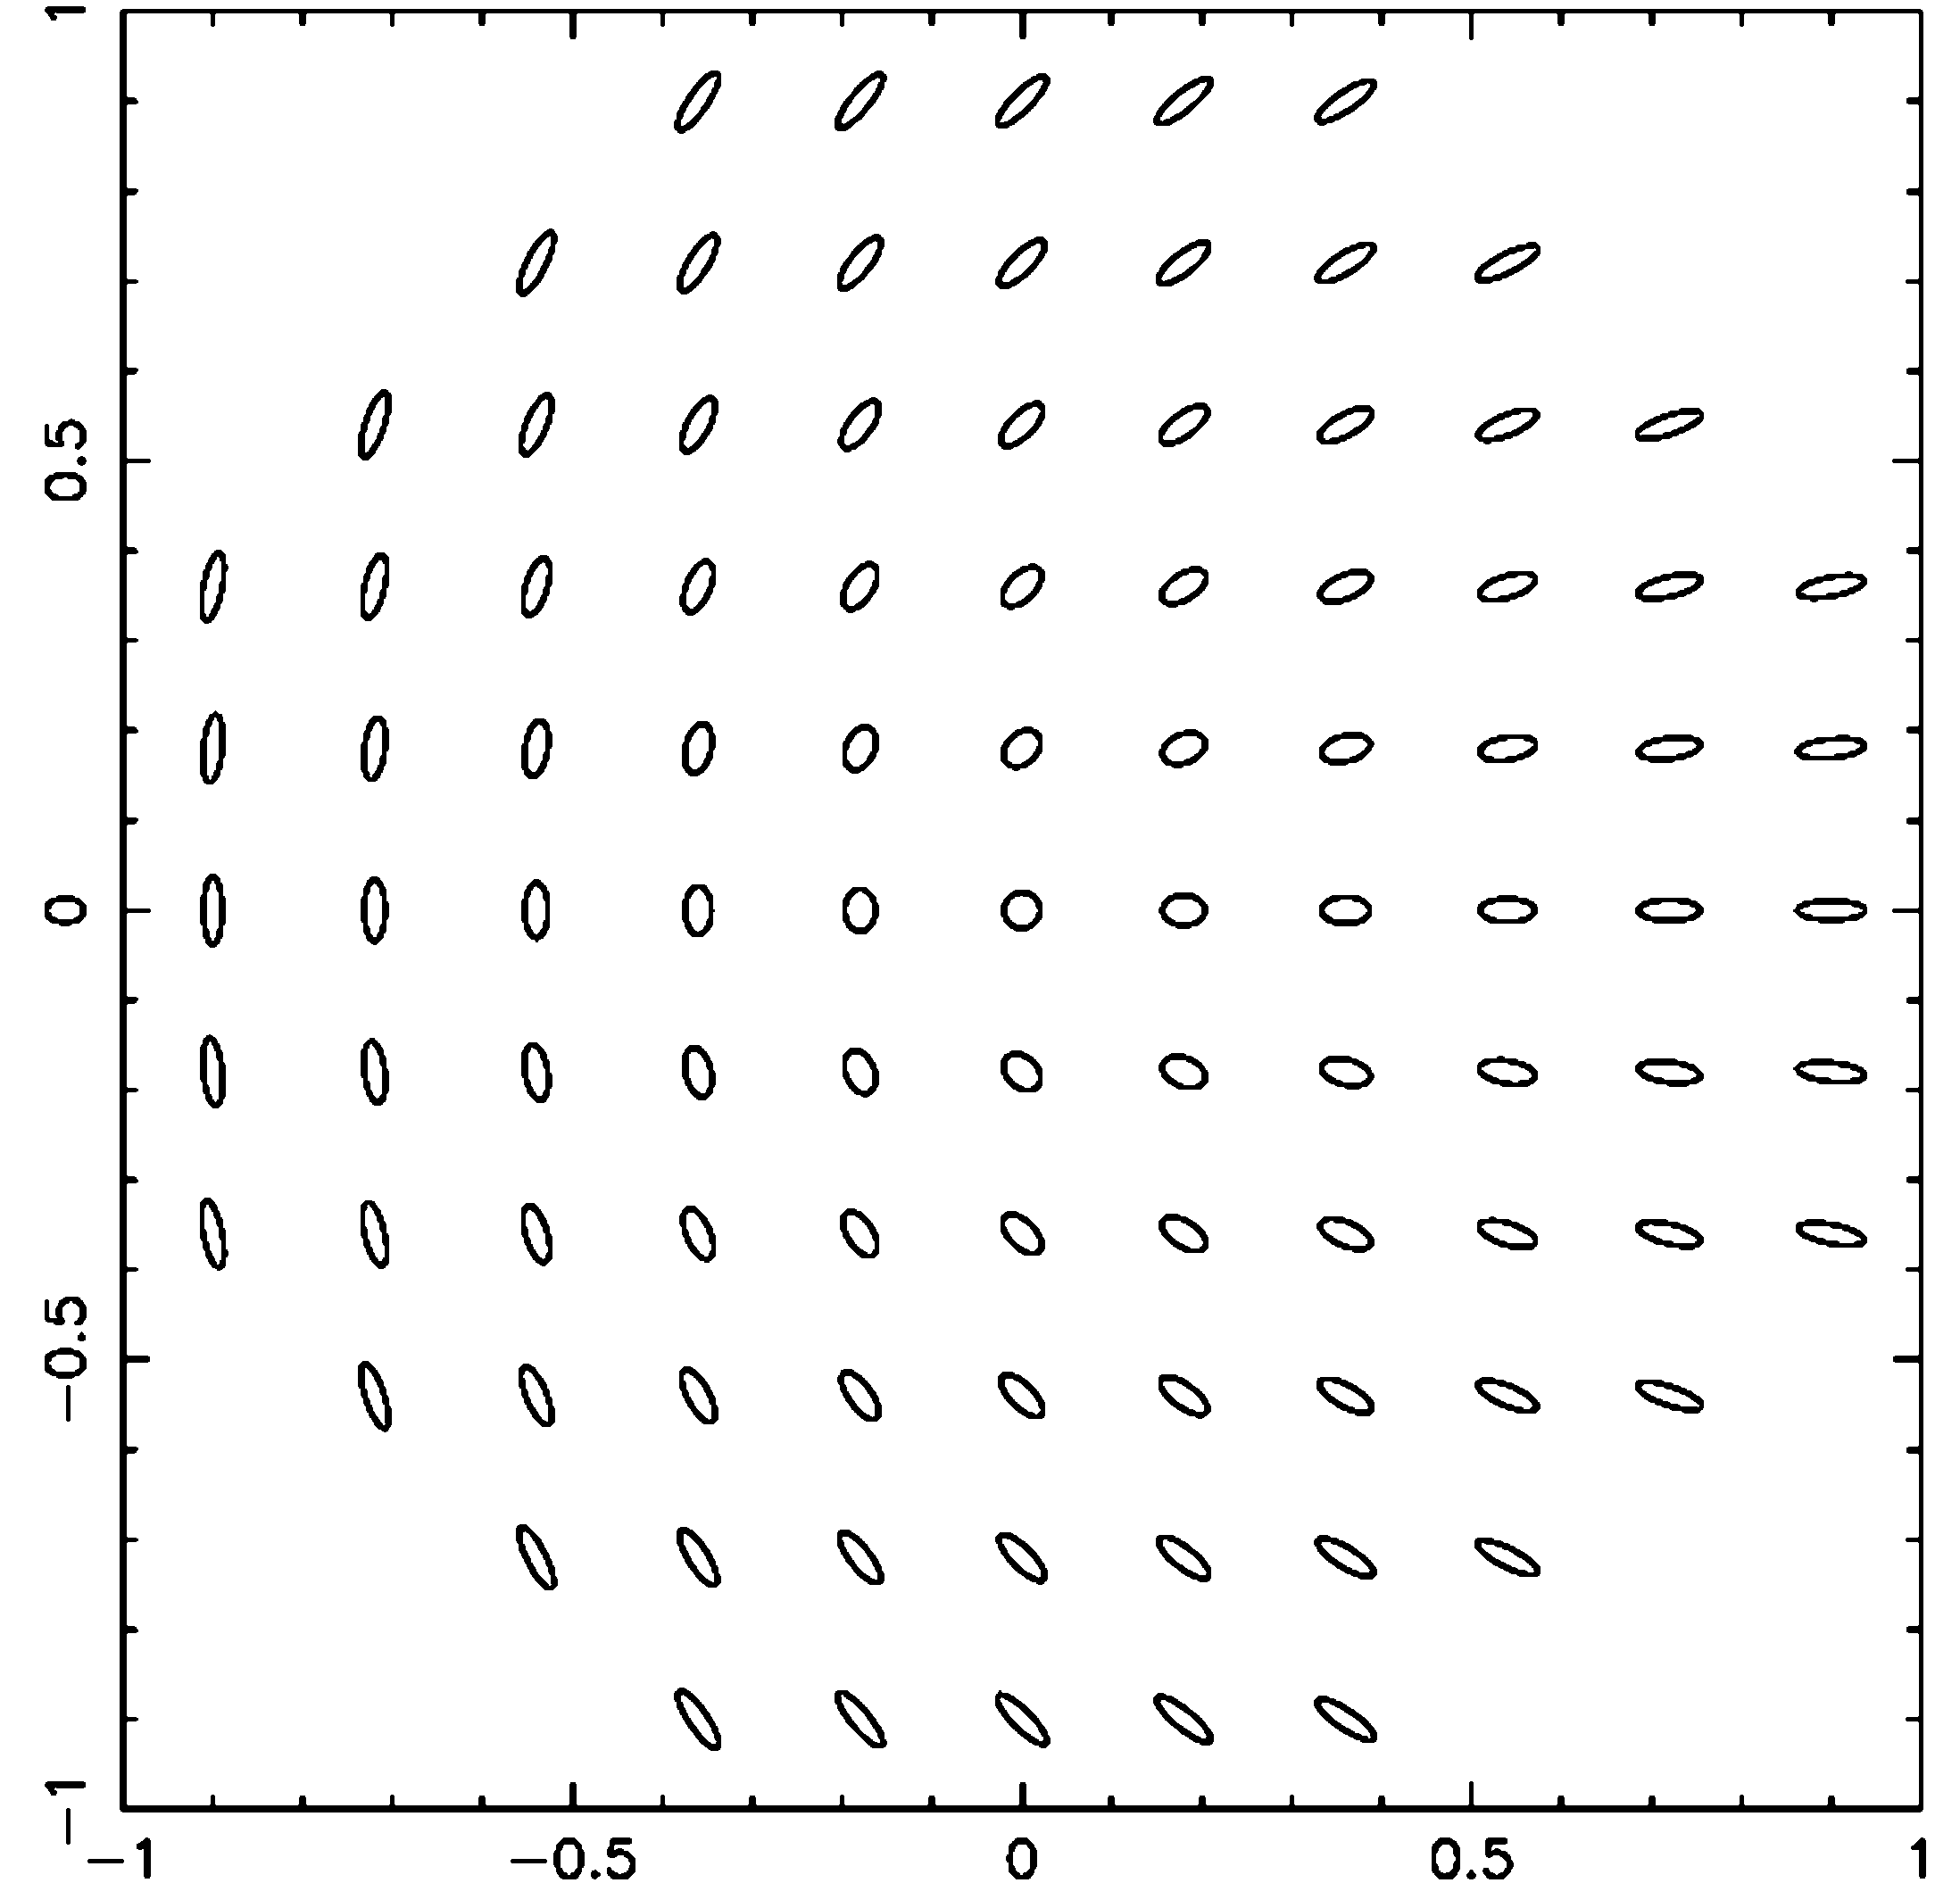
\includegraphics[width=\textwidth]{figs-swe/ellipse_orientations.png}
        \captionsetup{justification=raggedright,singlelinecheck=false}
        \caption{The shape of a galaxy image for various ellipticity components $\varepsilon_1$ and $\varepsilon_2$ on the $x$ and $y-$axes respectively. Taken from \cite{schneider}.}
        \label{ellipses}
    \end{subfigure}
    ~
    %% Einstein Ring Figure
    \begin{subfigure}[H]{0.425\textwidth}
        \includegraphics[width=\textwidth]{figs-swe/einstein_ring.png}
        \captionsetup{justification=raggedright,singlelinecheck=false}
        \caption{An image of the luminous red galaxy LRG 3-757 along with a strongy lensed background galaxy, called the `Cosmic Horseshoe'\cite{einstein_ring}}
        \label{einstein_ring}
    \end{subfigure}
    \caption{}
\end{figure*}

A full mathematical treatment of the gravitational lensing of galaxies due to the gravitational fields of massive objects requires general relativity (see \cite{modern_cosmology} for details). However, the important results can be summarized as follows. Foreground mass distorts the image of a background galaxy in two distinct ways: The image is magnified and sheared tangentially about the foreground mass, making it more elliptical. The magnification of the image is determined by the convergence $\kappa$, a scalar which measures the projected mass density along each line of sight. The shearing of the source is most often described by the complex shear $\gamma$ defined to be
\begin{equation}\label{complex_shear}
\gamma=\gamma_1+i\gamma_2=|\gamma|\,e^{2i\varphi}
\end{equation}

\noindent where $|\gamma|$ is the magnitude of the shear and $\varphi$ is the orientation of the shear. While the intrinsic ellipticities of source galaxies are randomly oriented near the foreground mass before lensing, they will be systematically more aligned with the shear field after lensing. Figure (??) demonstrates this process visually.

However, usually the quantity of interest in lensing calculations is the \textit{reduced} shear, defined by
\begin{equation}\label{reduced_shear}
g=\frac{\gamma}{1-\kappa}.
\end{equation}

\noindent Then using the thin lens approximation for the lensing of a background source of intrinsic ellipticity $\varepsilon_i$ around a point foreground mass with reduced shear $g$, the lensed ellipticity $\varepsilon$ is given by
\begin{equation}\label{lensing}
 \varepsilon = \begin{dcases} 
      \frac{\varepsilon_i+g}{1+g^*\varepsilon_i} & : |g|\leq1 \\[0.75em]
       \frac{1+g\varepsilon_i^*}{\varepsilon^*+g^*} & : |g|>1
   \end{dcases}
\end{equation}

\noindent where an asterisk denotes the complex conjugate\cite{schneider}. The behavior of the distortion relies strongly on the magnitude of $g$; the
effect is called \textit{strong} lensing if $|g|>1$ and \textit{weak} lensing if $|g|<1$. The effects of strong lensing can be quite dramatic, distorting sources into large arcs, multiple images, or even an Einstein ring as shown in Figure \ref{einstein_ring}. While strong lenses are rare as the alignment of the source and foreground mass must be nearly perfect, \textit{all} sources are weakly lensed. The effect is small, usually an ellipticity distortion of only a few percent (cite?), but can be detected locally by averaging the ellipticities of all sources in a small region. As the orientations of the sources should be random, it would be expected that
$$\left<\varepsilon\right>=0.$$

\noindent However, as sources in the same small region are sheared in (approximately) the same way, this implies that
\begin{equation}
\left<\varepsilon\right>\approx g.
\end{equation}

 \noindent Finally as in the weak lensing regime ${\kappa\ll1}$ and ${|\gamma|\ll1}$, it follows that
 \begin{equation}
 \gamma\approx g\approx\left<\varepsilon\right>
 \end{equation}

 \noindent which provides a method of detecting the shear observationally.

\subsection*{Dark Matter Halos}

While the exact relation between the distribution of galaxies and dark matter is not known, simulations have shown that galaxies tend to form in overdense regions of dark matter. This means that galaxies \textit{should} trace out the larger underlying dark matter structures. The simplest way to model this relationship is by enveloping each galaxy in a spherically symmetric dark matter `halo' of mass $M_h$ sampled from the stellar-to-halo mass relation\cite{smhr}. These halos extend far beyond the edge of the visible galaxy that they enclose. While the density profile of the halos may be complex, numerous simulations have shown that it can be well approximated by the Navarro-Frenk-White (NFW) profile which has the form
\begin{equation}\label{nfw_profile}
\rho_{NFW}(r)=\frac{\rho_0}{\frac{r}{R_s}\left(1+\frac{r}{R_s}\right)^2}
\end{equation}

\noindent where the constant $\rho_0$ and the scale radius $R_s$ are parameters that vary from halo to halo\cite{nfw}. This work uses a truncated NFW profile called the Baltz-Marshall-Oguri (BMO) profile given by
\begin{equation}\label{bmo_profile}
\rho_{BMO}(r)=\rho_{NFW}\cdot\left(\frac{r_t^2}{r^2+r_t^2}\right)^2
\end{equation}

\noindent where $r_t$ is a free parameter, as it has been shown to be a better fit to simulated data\cite{nfw_bmo}.

\section{The Pangloss Framework}

%% Pangloss Cartoon
\begin{figure*}
    \centering
    \includegraphics[width=0.85\textwidth]{figs-swe/pangloss_cartoon.png}
    \captionsetup{justification=raggedright,singlelinecheck=false}
    \caption{A cartoon model of how the \texttt{Pangloss} framework uses a dark matter halo model to reconstruct the foreground mass along the line of sight of a background source galaxy. The shear and convergence at the line of sight contributed by each halo is calculated, and the predicted ellipticity is calculated using the sum of these contributions.}
    \label{pangloss_cartoon}
\end{figure*}

To constrain the mass of foreground dark matter using weak gravitational lensing, first a model of the relationship between foreground galaxies and the foreground dark matter must be established and robustly tested to see if, statistically, it makes the same lensing predictions of background sources as the true undering dark matter structure. To do this, I built upon the publically available \texttt{Pangloss} framework used in Collett et al.\cite{collett_marshall} to reconstruct all the mass along the line of sight of each background galaxy using dark matter halos. The lensing contribution of each halo is calculated, and the total lensing of the background galaxy is the sum of each halo contribution. This process is detailed in the following sections.

\subsection*{Assumptions}
While \texttt{Pangloss} may be used more generally, the present analysis makes some additional strong assumptions to simplify the problem for a first attempt at making weak lensing predictions.

\begin{enumerate}
\item The dark matter mass distribution can be approximated by spherically symmetric BMO halo profiles attached to each galaxy.
\item The stellar mass of the foreground galaxy is negligible for lensing calculations.
\item The mass of the dark matter halo of each foreground galaxy is known.
\item A spectroscopic redshift of each foreground galaxy is known.
\end{enumerate}

Testing the first assumption is the main goal of this paper. The second assumption is reasonable as it is estimated that dark matter halos are 1-2 orders of magnitude more massive than the host galaxy\cite{smhr}. Clearly the third assumption will never be true for any observational data. However, this allows for a best-case scenario estimate of how well the \texttt{Pangloss} framework \textit{could} predict weak lensing effects given all possible information. This assumption can be relaxed by sampling a dark matter halo mass from an assumed stellar mass - halo mass relation. The fourth assumpition is also unrealistic as most galaxies in sky surveys only have a less-reliable photometric redshift due to time constraints, but this again allows for a best-case estimate. This assumption could be relaxed by instead using photometric redshifts, adding random noise, and repeating the upcoming analysis on many realizations of the photometric redshifts.

\subsection*{The Millennium Simulation}
\texttt{Pangloss} cannot be used to make dark matter mass maps using existing galaxy catalogs until it is tested on a simulated universe with known dark matter structure to determine how accurately and precisely it predicts the lensing of background sources. For this purpose, \texttt{Pangloss} was tested on galaxy catalogs from the Millennium Simulation, an N-body simulation consisting of over 10 billion dark matter `particles' each representing a billion solar masses and populated with about 20 million galaxies\cite{millennium_simulation}. The simulation uses cosmological parameters from WMAP 1\textsuperscript{st}-year data analysis and contains baryonic and dark matter structure believed to be consistent with our own universe. From the work of Hilbert et al.\cite{ray_tracing}, high resolution maps of the shear and convergence from the perspective of a single reference point calculated by ray-tracing are publically available. From these maps, the actual lensing of background galaxies when traveling through the foreground mass of the Millennium Simulation towards the reference point can be calculated using Equation \eqref{lensing}.

\subsection*{Generating Background Galaxies}
With a catalog of foreground galaxies chosen, a set of background galaxies with density 10 per arcminute$^2$ was generated. The intrinsic orientation of each galaxy was sampled from a uniform distribution as, without lensing, there should be no preferred orientation due to the assumption of an isotropic universe. The magnitude of the galaxy ellipticities was sampled from a normal distribution with a standard deviation of 0.2, but any ellipticities with magnitude greater than one were re-sampled. Random ellipticity noise was sampled from a normal distribution with a standard deviation of 0.1 and added to the intrinsic ellipticities. Finally, each ellipticity was multiplied by $M=0.9$ to account for a multiplicative bias of 10\%.

\subsection*{Creating Lightcones}

While ideally all foreground mass in a field would be considered when predicting the weak lensing of a background galaxy, it is computationally prohibitive to do so. Instead, all foreground halos contained within a `lightcone' centered along the line of sight to the source and extending out to a chosen lightcone radius $R$ were considered when calculating the lensing contributions for the background source. A cartoon model of this process is shown in Figure \ref{pangloss_cartoon}. Unless otherwise specified, experiments in this paper used a radius of 2 arcminutes.

To calculate the convergence and shear contribution of each halo, the physical distance from the halo to the line of sight was needed. To increase the speed of distance calculations, the foreground halo redshifts were first snapped to a grid of 100 equally-sized redshift bins and then converted to physical distance.

Using the physical separation distance and halo mass, the shear and convergence contribution of a single foreground halo is calculated using methods described in Wright and Brainerd\cite{lensing_calc}. The total convergence and shear at the center of the lightcone is simply the sum of the convergence and shear contributions of each halo contained in the lightcone. The \texttt{Pangloss}-predicted lensed background ellipticity is then calculated using Equation \eqref{lensing}.

\subsection*{Checking the Halo Model}

Instead of comparing the ray-traced and \texttt{Pangloss}-predicted ellipticities for individual galaxies, the lensing is characterized globally with correlation functions. The ellipticity-ellipticity correlation function measures how correlated the ellipticities of pairs of galaxies are as a function of separation distance, while the galaxy-mass correlation function measures the correlation of lensed ellipticities around foreground halos as a function of separation distance. For readers that are unfamiliar with correlation functions in the context of cosmology or want a visual aid, see Appendix A. Both correlation functions are used in this work to measure how well the \texttt{Pangloss} framework models weak lensing by dark matter structures using the publically available \texttt{TreeCorr} module written by Mike Jarvis (website url?). Note that the correlation function definition used in \texttt{TreeCorr} is slightly different than that used in most of the literature; for a derivation of the connection between Jarvis's definition and the more common Schneider definition\cite{schneider}, see Appendix B.

\section{Results}

Using the presented methodology, (x \# of background sources) background galaxies in a (y*y square deg) subset of the (0,0,0,0) Millennium Simulation foreground catalog (cite where to get data) were generated and lensed by both the ray-traced shear and convergence maps as well as the \texttt{Pangloss} framework. On average, the lightcones contained (950??)$\pm$(25??) foreground halos. Both sets of lensed ellipticities were characterized with correlation functions, as well as the intrinsic ellipticities of the sources before lensing.

\subsection*{Ellipticity-Ellipticity Correlation Function}

The first test of the halo model was with the ellipticity-ellipticity correlation function with a lightcone radius of 2 arcminutes which is given in Figure \ref{gg_corr}. The statistic measured the average correlation between pairs of ellipticities at separation distances between (0.1??) arcminutes and 2 arcminutes. The correlation function of the intrinsic ellipticities plotted in blue shows no significant deviation from zero as expected, as before lensing the galaxies had random orientations. Both the ray-traced, plotted in green, and halo model, plotted in purple, ellipticities show positive correlation on small scales up to a separation of 0.8 arcminutes. However, the ray-traced correlation is positive on all calculated scales while the halo model does not predict any significant corrlelation at separations above 0.8 arcminutes. Additionally, while the shapes of the correlation functions for both sets of lensed ellipticities aggree well until 0.8 arcminutes, there is a clear systematic underprediction of shear power by the halo model on all scales. On average, the shear power is underpredicted by (??) percent.

%% Ellipticity-Ellipticity Correlation
\begin{figure}
    \centering
    \begin{subfigure}[h]{0.475\textwidth}
        \includegraphics[width=\textwidth]{figs-swe/gg_corr.png}
        \captionsetup{justification=raggedright,singlelinecheck=false}
        \caption{The ellipticity-ellipticity correlation function for (x \# of bg) sources at separation distances from 0.1 arcminutes to 2 arcminutes and a lightcone radius of $R=2$ arcminutes. While the correlation of the intrinsic ellitpicities before lensing (blue) shows no correlation, the correlation of the ray-traced ellipticities (green) and halo model predicted ellipticities (purple) both show significant positive correlation on scales up to 0.8 arcminutes. The halo model predicts no correlation above this scale, while the ray-tracing shows positive correlation on all scales.}
        %The correlation of the intrinsic ellitpicities before lensing is plotted in blue, and shows no correlation. The correlation of the true ray-traced ellipticities is plotted in green and shows significant positive correlation on all scales. The halo predicted correlation, plotted in purple, shows significant positive correlation until a separation distance of 0.8 arcminutes.
        \label{gg_corr}
    \end{subfigure}
    ~~
    \begin{subfigure}[h]{0.475\textwidth}
        \includegraphics[width=\textwidth]{figs-swe/gg_corr_series.png}
        \captionsetup{justification=raggedright,singlelinecheck=false}
        \caption{The ellipticity-ellipticity correlation functions for a series of halo model frameworks with increasing lightcone radii from $R=1$ arminute to $R=8$ arcminutes, all plotted in purple with various line styles. These are compared to the ray-traced correlation using a radius of 2 arcminutes plotted in green.}
        \label{gg_corr_series}
    \end{subfigure}
    \caption{}
\end{figure}


Using the same catalog of background sources, this statistic was recalculated for the ray-traced and halo model lensed ellipticities for various lightcone radii ranging from $R=1$ arcminute to $R=???$ arcminutes. The result is shown in Figure \ref{gg_corr_series}.

(Analysis of plot)

\subsection*{Galaxy-mass Correlation Function}

The catalog of lensed ellipticities was also analyzed using the galaxy-mass correlation function with separation distances from (0.1??) arcminutes to 2 arcminutes and a lightcone radius of 2 arcminutes. The result is shown in Figure (??). As with the ellipticity-ellipticity correlation function, there is no significant correlation for the intrinsic ellipticities at any scale as expected. The lensed ellipticities from the ray-tracing and halo model both have positive correlation on all calculated scales and are in agreement on scales from (??) arcminutes to (??) arcminutes. However, the halo model is still systematically underpredicting the shear power on scales above (??) arcminutes, although now only by an average of (??) percent. A new feature is the large overprediction of shear power on separation scales smaller than (??) arcminutes. However, background sources this close to foreground halos are often in the strong lensing regime which is not currently accounted for by the \texttt{Pangloss} framework.

%% Galaxy-mass correlation function
\begin{figure}
    \centering
    \includegraphics[width=0.475\textwidth]{figs-swe/ng_corr.png}
    \captionsetup{justification=raggedright,singlelinecheck=false}
    \caption{The galaxy-mass correlation function of (x \# of bg) sources at separation distances from 0.1 arcminutes to 2 arcminutes and a lightcone radius of $R=2$ arcminutes. There is no significant correlation of the intrinsic ellipticities (blue) as expected, and both the ray-traced corrleation (green) and halo model correlation (purple) are positive on all scales. The green and purple curves are in agreement from 0.? to 0.? arcminutes, but have significant discrepancies on scales above and below this range.}
    \label{pangloss_cartoon}
\end{figure}
(Make a plot of n-g correlation function with multiple R's?? - No, mention that it was made but does not contain any interesting results)

\subsection*{Computational Performance}

A secondary goal of this research was to investigate how quickly the prediction for the shear and convergence for a single background source could be made. The average CPU time required for the prediction per lightcone was (80? $\pm$ 10?) ms for the first run. However, many small improvements to the coding infastructure of \texttt{Pangloss} were made to speed up the prediction. The average CPU time for a lensing prediction per lightcone after various changes is plotted in Figure (??).

%************************
(CPU time per lightcone plot)\\
%************************
(Include RAM in plot??)

\section{Discussion}

\subsection*{Issues with the \texttt{Pangloss} Framework}

Both the ellipticity-ellipticity and galaxy-mass correlation functions show clear issues with using the halo model to predict the lensing of background sources with \texttt{Pangloss}, even in the best-case scenario of perfect knowledge of the halo masses and their spectroscopic redshifts. The systematic underprediction of shear power present in both correlaton functions is likely do to missing features in the model such as clusters, filaments, and voids. 

While individual galaxies currently recieve halos, a cluster of galaxies will sit in an larger halo whose presence is not being considered as its position, mass, and extent are difficult to determine. The absence of this mass undoubtedly effects shear predictions and ellipticity correlations on large scales. While some of the filament structure is captured in the framework, as the higher density of galaxies in filaments will lead to a higher density of halos, any additional dark matter structure between halos and clusters is not being accounted for. While difficult to do in practice, one can imagine connecting clusters of galaxies with dark matter `cylinders' to account for the extra filament mass. Voids are also not currently considered, as the framework assumes the field has constant mass density equal to that of the average mass density of the universe and then adds halo masses on top of this density. This would make the average matter density accross the field \textit{larger} than the mean density of the unvierse, and could be counteracted by subtracting mass from regions in between foreground halos. Stellar masses could also be incorperated into the \texttt{Pangloss} prediction, but any effect would likely be dominated by the missing features described above.

The progression of model-predicted ellipticity-ellipticity correlation functions at larger radii converging to the ray-traced correlation supports the analysis given above, as the prediction was progressively better with larger number of foreground halos and thus more mass and structure. However, the number of foreground objects scales quadratically with the lightcone radius making it prohibitively expensive above $R=8$ arcminutes. With a radius this large, most foreground objects will be too far away from the line of sight and have insufficient mass to make a significant contribution to the lensing of the background source. This suggests the creation of a metric to predict the `relevance' of each halo to the lensing contribution. In this way, the framework could be restructured to only use the most relevant halos in the computationally expensive lensing prediction, while simultaneously allowing for larger lightcones with more relevant halos. This could aid in the aforementioned shear power prediction issues.  

\subsection*{Scaling Up \texttt{Pangloss}}

While the current \texttt{Pangloss} framework can handle the lensing predictions of (x \# of lightcones) in a (y*y square degree) field comfortably on a single processor, the goal is to scale up the framework to make predictions for background sources of the same number density in a 100 deg$^2$ field; this will require 3.6 million lightcones, each containing up to 1,000 foreground halos. Luckily, the prediction is trivially parallelizable as the shear and convergence calculation of each lightcone is independent of all other lightcones. This makes GPUs an attractive candidate for future work, as it would only take 360 GPUs with 10,000 threads each to carry out the prediction. Additionally, the (??) MB of RAM per lightcone is sufficiently small to fit 10,000 lightcones on a GPU.

\section{Conclusion}

A simple halo model was used to reconstruct the mass along line of sights in the Millennium Simulation to make predictions of how the foreground mass weakly lensed the ellipticities of (x \# of bg) of generated background sources. The lensed ellipticities were characterized globally using the ellipticity-ellipticity and galaxy-mass correlation functions and compared to the ray-traced correlations.

\section{Acknowledgements}

I would like to thank the Department of Energy's Science Undergraduate Laboratory Internship (SULI) program for funding this research and giving me the opportunity to conduct research at ?. asdf. Finally, I am incredibly grateful to Phil Marshall for his unending support, patience, and guidance throughout this research.

This work was supported in part by the U.S. Department of Energy, Office of Science, Office of Workforce Development for Teachers and Scientists (WDTS) under the Science Undergraduate Laboratory Internships Program (SULI).

\begin{itemize}
\item DOE
\item SULI
\item Stanford University
\item KIPAC
\item Risa, Matt, Pat
\item Phil!!
\end{itemize}

\onecolumngrid

\section{References}

\bibliographystyle{plain}
\bibliography{suli-report-swe}

\section{Appendix}

\subsection{Visualizing Correlation Functions}

\begin{itemize}
\item Use as a brief introduction to the shear-shear and galaxy-mass correlation function as used in this work
    \begin{itemize}
    \item reference other (much more detailed) material for readers to find
    \end{itemize}
\item Include correlation value colormaps for $\xi_+$, $\xi_-$, and $\xi_\times$ along with discussion of correlation pattern
\item Include color-coded correlation visuals along with setup
    \begin{itemize}
    \item Galaxies around lens before lensing - correlation values scatter plot with no signal
    \item Galaxies around lens after lensing - correlation values scatter plot with signal
    \end{itemize}
\item B-modes and E-modes plot??
\end{itemize}

\subsection{Jarvis Proof}

\begin{itemize}
\item Introduction to difference between the common Schneider definition of lensing correlation functions and that used by Jarvis`s \texttt{TreeCorr} code
\item Here we derive the connection between the two
\item Definitions of each, along with references
\end{itemize}

From Jarvis \href{http://arxiv.org/pdf/astro-ph/0307393v2.pdf}{(Page 3)}:
\begin{align}
\xi_+&=\left<\gamma_i\gamma_j^*\right>=\texttt{xip}+i(\texttt{xip\_im})\label{s+}\\
\xi_-&=\left<\gamma_i\gamma_je^{-4i\alpha}\right>=\texttt{xim}+i(\texttt{xim\_im})\label{s-}
\end{align}

where $\alpha$ is the angle between the two objects $i,j$ and each $\gamma$ is given by $\gamma_n=|\gamma_n|e^{2i\theta_n}$ in polar form.\\

From Schneider \href{http://arxiv.org/pdf/astro-ph/0509252v1.pdf}{(Page 92)}:
\begin{align}
\xi_\pm&=\left<\gamma_{i_t}\gamma_{j_t}\right>\pm\left<\gamma_{i_\times}\gamma_{j_\times}\right>\label{s+-}\\
\xi_\times&=\left<\gamma_{i_t}\gamma_{j_\times}\right>\label{sx}
\end{align}

where $\gamma_{n_t}=-\operatorname{Re}\left(\gamma_n e^{-2i\alpha}\right)$ and $\gamma_{n_\times}=-\operatorname{Im}\left(\gamma_n e^{-2i\alpha}\right)$.\\

\section*{Schneider's $\xi_+$ to Jarvis's \texttt{xip}}

Starting with Schneider's definition, observe that
\begin{align*}
\xi_+&=\left<\gamma_{i_t}\gamma_{j_t}\right>+\left<\gamma_{i_\times}\gamma_{j_\times}\right>\\
&=\left<\operatorname{Re}\left(\gamma_ie^{-2i\alpha}\right)\cdot\operatorname{Re}\left(\gamma_je^{-2i\alpha}\right)\right>+\left<\operatorname{Im}\left(\gamma_ie^{-2i\alpha}\right)\cdot\operatorname{Im}\left(\gamma_je^{-2i\alpha}\right)\right>\\
&=\left<\operatorname{Re}\left(|\gamma_i|e^{2i(\theta_i-\alpha)}\right)\cdot\operatorname{Re}\left(|\gamma_j|e^{2i(\theta_j-\alpha)}\right)\right>+\left<\operatorname{Im}\left(|\gamma_i|e^{2i(\theta_i-\alpha)}\right)\cdot\operatorname{Im}\left(|\gamma_j|e^{2i(\theta_j-\alpha)}\right)\right>\\
&=\left<|\gamma_i|\cdot|\gamma_j|\cos\left(2(\theta_i-\alpha)\right)\cos\left(2(\theta_j-\alpha)\right)\right>+\left<|\gamma_i|\cdot|\gamma_j|\sin\left(2(\theta_i-\alpha)\right)\sin\left(2(\theta_j-\alpha)\right)\right>.
\end{align*}

Using the trig identities
\begin{align}
\cos(u)\cos(v)&=\frac{1}{2}\left[\cos(u-v)+\cos(u+v)\right],\\
\sin(u)\sin(v)&=\frac{1}{2}\left[\cos(u-v)-\cos(u+v)\right],
\end{align}

and the linearity of the expectation operator, it is straightforward to show that
%\begin{align*}
%\xi_+&=\left<|\gamma_i|\cdot|\gamma_j|\right>\cdot\left(\left<\frac{1}{2}\left[\cos\left(2(\theta_i-\theta_j)\right)+\cos\left(2(\theta_i+\theta_j-2\alpha)\right)\right]\right>+\left<\frac{1}{2}\left[\cos\left(2(\theta_i-\theta_j)\right)-\cos\left(2(\theta_i+\theta_j-2\alpha)\right)\right]\right>\right)\\
%&=\left<|\gamma_i|\cdot|\gamma_j|\cos\left(2(\theta_i-\theta_j)\right)\right>.
%\end{align*}
$$\xi_+=\left<|\gamma_i|\cdot|\gamma_j|\cos\left(2(\theta_i-\theta_j)\right)\right>.$$

Now using the identity
\begin{equation}\label{trig2}
\cos(u\pm v)=\cos\left(u\right)\cos\left(v\right)\mp\sin\left(u\right)\sin\left(v\right),
\end{equation}

the previous equation can be written as

\begin{align*}
\xi_+&=\left<|\gamma_i|\cdot|\gamma_j|\cdot\left[\cos\left(2\theta_i\right)\cos\left(2\theta_j\right)+\sin\left(2\theta_i\right)\sin\left(2\theta_j\right)\right]\right>\\
&=\left<\operatorname{Re}(\gamma_i)\cdot\operatorname{Re}(\gamma_j)+\operatorname{Im}(\gamma_i)\cdot\operatorname{Im}(\gamma_j)\right>.
\end{align*}

Using the complex number identities

\begin{align}
\operatorname{Re}(z)&=\frac{1}{2}\left[z+z^*\right],\label{complex1}\\
\operatorname{Im}(z)&=\frac{1}{2i}\left[z-z^*\right]\label{complex2},
\end{align}

it follows that

\begin{align*}
\xi_+&=\left<\frac{1}{4}\left[(\gamma_i+\gamma_i^*)(\gamma_j+\gamma_j^*)-(\gamma_i-\gamma_i^*)(\gamma_j-\gamma_j^*)\right]\right>\\
&=\left<\frac{1}{2}\left[\gamma_i\gamma_j^*+(\gamma_i\gamma_j^*)^*\right]\right>\\
&=\left<\operatorname{Re}(\gamma_i\gamma_j^*)\right>=\texttt{xip}.
\end{align*}

\section*{Schneider's $\xi_-$ to Jarvis's \texttt{xim}}

The first few steps are identical to the previous section besides the negative in the definition of $\xi_-$, giving
\begin{align*}
\xi_-&=\left<\gamma_{i_t}\gamma_{j_t}\right>-\left<\gamma_{i_\times}\gamma_{j_\times}\right>\\
&=\left<|\gamma_i|\cdot|\gamma_j|\cos\left(2(\theta_i-\alpha)\right)\cos\left(2(\theta_j-\alpha)\right)\right>-\left<|\gamma_i|\cdot|\gamma_j|\sin\left(2(\theta_i-\alpha)\right)\sin\left(2(\theta_j-\alpha)\right)\right>\\
&=\left<|\gamma_i|\cdot|\gamma_j|\cos\left(2(\theta_i+\theta_j-2\alpha)\right)\right>.
\end{align*}

Now using Equation \eqref{trig2} twice, first letting $u=2(\theta_i+\theta_j)$ and $v=-4\alpha$, and then letting $u=2\theta_i$ and $v=2\theta_j$, this equation becomes

\begin{align*}
\xi_-&=\left<|\gamma_i|\cdot|\gamma_j|\Big(\left[\cos(2\theta_i)\cos(2\theta_j)-\sin(2\theta_i)\sin(2\theta_j)\right]\cos(4\alpha)+\left[\sin(2\theta_i)\cos(2\theta_j)+\cos(2\theta_i)\sin(2\theta_j)\right]\sin(4\alpha)\Big)\right>\\
&=\Big<\big[\operatorname{Re}(\gamma_i)\cdot\operatorname{Re}(\gamma_j)-\operatorname{Im}(\gamma_i)\cdot\operatorname{Im}(\gamma_j)\big]\cos(4\alpha)+\big[\operatorname{Im}(\gamma_i)\cdot\operatorname{Re}(\gamma_j)+\operatorname{Re}(\gamma_i)\cdot\operatorname{Im}(\gamma_j)\big]\sin(4\alpha)\Big>.
\end{align*}

Using the identities \eqref{complex1} and \eqref{complex2}, and simplifying the leftover terms, this equation can be shown to equal
\begin{align*}
\xi_-=\big<\operatorname{Re}(\gamma_i\gamma_j)\cos(4\alpha)+\operatorname{Im}(\gamma_i\gamma_j)\sin(4\alpha)\big>.
\end{align*}

Now observe that for two complex numbers $a$ and $b$, it is true that

$$\operatorname{Re}(a\cdot b^*)=\operatorname{Re}(a)\cdot\operatorname{Re}(b)+\operatorname{Im}(a)\cdot\operatorname{Im}(b).$$

Then setting $a=\gamma_i\gamma_j$ and $b=e^{4i\alpha}$, it must be true that

$$\operatorname{Re}\left(\gamma_i\gamma_je^{-4i\alpha}\right)=\operatorname{Re}(\gamma_i\gamma_j)\cos(4\alpha)+\operatorname{Im}(\gamma_i\gamma_j)\sin(4\alpha).$$

Combining this with our previous result, this means that

$$\xi_-=\big<\operatorname{Re}(\gamma_i\gamma_j)\cos(4\alpha)+\operatorname{Im}(\gamma_i\gamma_j)\sin(4\alpha)\big>=\left<\operatorname{Re}\left(\gamma_i\gamma_je^{-4i\alpha}\right)\right>=\texttt{xim}.$$

\section*{Schneider's $\xi_\times$ to Jarvis's $\frac{1}{2}\left(\texttt{xim\_im}-\texttt{xip\_im}\right)$}

Starting from Schneider's definition of $\xi_\times$,

\begin{align*}
\xi_\times&=\left<\gamma_{i_t}\gamma_{j_\times}\right>\\
&=\left<\operatorname{Re}\left(|\gamma_i|e^{2i(\theta_i-\alpha)}\right)\cdot\operatorname{Im}\left(|\gamma_j|e^{2i(\theta_j-\alpha)}\right)\right>\\
&=\big<|\gamma_i|\cdot|\gamma_j|\cos\left(2(\theta_i-\alpha)\right)\sin\left(2(\theta_j-\alpha)\right)\big>.\\
\end{align*}

Using the trig identity

\begin{equation}\label{trig3}
\cos(u)\sin(v)=\frac{1}{2}\left[\sin(u+v)-\sin(u-v)\right],
\end{equation}

the previous equation becomes

\begin{align*}
\xi_\times&=\left<|\gamma_i|\cdot|\gamma_j|\cdot\frac{1}{2}\big[\sin\left(2(\theta_i+\theta_j-2\alpha)\right)-\sin\left(2(\theta_i-\theta_j)\right)\big]\right>.
\end{align*}

Next, applying the identities

\begin{equation}\label{trig4}
\sin(u\pm v)=\sin(u)\cos(v)\pm\cos(u)\sin(v)
\end{equation}

along with \eqref{trig2} iteratively until each trig function only has a single term, the equation becomes

\begin{align*}
\xi_\times&=\Big<|\gamma_i|\cdot|\gamma_j|\cdot\frac{1}{2}\Big(\left[\sin(2\theta_i)\cos(2\theta_j)+\cos(2\theta_i)\sin(2\theta_j)\right]\cos(4\alpha)\\
&\qquad\qquad\qquad\quad-\left[\cos(2\theta_i)\cos(2\theta_j)-\sin(2\theta_i)\sin(2\theta_j)\right]\sin(4\alpha)\\
&\qquad\qquad\qquad\quad-\sin(2\theta_i)\cos(2\theta_j)+\cos(2\theta_i)\sin(2\theta_j)\Big)\Big>\\
&=\Big<\frac{1}{2}\Big(\left[\operatorname{Im}(\gamma_i)\cdot\operatorname{Re}(\gamma_j)+\operatorname{Re}(\gamma_i)\cdot\operatorname{Im}(\gamma_j)\right]\cos(4\alpha)\\
&\qquad-\left[\operatorname{Re}(\gamma_i)\cdot\operatorname{Re}(\gamma_j)-\operatorname{Im}(\gamma_i)\cdot\operatorname{Im}(\gamma_j)\right]\sin(4\alpha)\\
&\qquad-\operatorname{Im}(\gamma_i)\operatorname{Re}(\gamma_j)+\operatorname{Re}(\gamma_i)\cdot\operatorname{Im}(\gamma_j)\Big)\Big>.\\
\end{align*}

Using the identities \eqref{complex1} and \eqref{complex2}, this can be simplified to

\begin{align*}
\xi_\times&=\left<\frac{1}{2}\big[\operatorname{Im}(\gamma_i\gamma_j)\cos(4\alpha)-\operatorname{Re}(\gamma_i\gamma_j)\sin(4\alpha)-\operatorname{Im}(\gamma_i\gamma_j^*)\big]\right>.
\end{align*}

Consider again two complex numbers $a$ and $b$. Observe that

$$\operatorname{Im}(a\cdot b^*)=\operatorname{Im}(a)\cdot\operatorname{Re}(b)-\operatorname{Re}(a)\cdot\operatorname{Im}(b).$$

Then setting $a=\gamma_i\gamma_j$ and $b=e^{4i\alpha}$, it must be true that

$$\operatorname{Im}\left(\gamma_i\gamma_je^{-4i\alpha}\right)=\operatorname{Im}(\gamma_i\gamma_j)\cos(4\alpha)-\operatorname{Re}(\gamma_i\gamma_j)\sin(4\alpha).$$

Combing these results give

\begin{align*}
\xi_\times&=\left<\frac{1}{2}\big[\operatorname{Im}(\gamma_i\gamma_j)\cos(4\alpha)-\operatorname{Re}(\gamma_i\gamma_j)\sin(4\alpha)-\operatorname{Im}(\gamma_i\gamma_j^*)\big]\right>\\
&=\left<\frac{1}{2}\big[\operatorname{Im}\left(\gamma_i\gamma_je^{-4i\alpha}\right)-\operatorname{Im}(\gamma_i\gamma_j^*)\big]\right>\\
&=\frac{1}{2}\big[\texttt{xim\_im}-\texttt{xip\_im}\big].
\end{align*}

as desired.

\end{document}
%
% ****** End of file apssamp.tex ******

\end{document}



% Outline:

%% Introduction:
\begin{itemize}
\item Broad intro into cosmology and dark matter, set problem in context
    \begin{itemize}
    \item (Very) short introduction to history of dark matter, Zwicky, rotation curves, etc.
    \end{itemize}
\begin{itemize}
\item Introduction to gravitational lensing
    \begin{itemize}
    \item Convergence and Shear / Strong and Weak lensing
        \begin{itemize}
        \item Dramatic effect of strong lensing, how it is used for constraining cos. parameters
        \item Only a few hundred known, not good for making mass maps
        \item All galaxies are weakly lensed, good for our purposes
        \end{itemize}
    \end{itemize}
\end{itemize}
\item What this work does and aims for
\begin{itemize}
    \item We aim to implement a simple dark matter halo model to predict weak-lensing effects by foreground mass - and to make the prediction `quickly' and/or with large parallelization
    \item Quick summary of what we do in paper
        \begin{itemize}
        \item Use halo model to make approximation of dark matter mass distribution in Millennium Simulation
        \item Use shear-shear and galaxy-mass correlation functions as summary statistics
        \item Compare statistics to ray-traced data
        \item Discuss physial and computational shortcomings with current methodology
        \end{itemize}
    \end{itemize}
\end{itemize}

%% Theoretical Background:
\begin{itemize}
\item Galaxy ellipticities
    \begin{itemize}
    \item (Most) galaxies are not circular - have intrinsic ellipticities
        \begin{itemize}
        \item If they were all circular, we could measure the change in shape exactly!
        \end{itemize}
    \item Galaxies are not always well approximated by ellipses (reference)
    \item Mathematical formalism
    \item Plot of galaxy orientation given e1 and e2 from P.J. Marshall thesis
    \end{itemize}
\item Shape noise and PSF issues in weak lensing (distorting already weak signal)
\item Gravitational lensing
    \begin{itemize}
    \item Short introduction to problem setup for simple case (point mass maybe?)
    \item Assumptions made in a typical solution (thin lens approximation?)
    \item Show solution from Schneider
    \item Shear and convergence 
    \item Measuring shear in weak lensing - a statistical feature
    \end{itemize}
\item Dark matter halos
    \begin{itemize}
    \item NFW profile and equation (reference)
    \item BMO truncation and equation (reference)
    \end{itemize}
\item SMHR? Or too distracting?
\end{itemize}

% Old theory:
%However, the important results for a point mass using the thin lens approximation can be summarized as follows: The distortion of a background galaxy image can be quantified by the linearized lens mapping Jacobi matrix $\mathcal{A}$ which can be written as

%$$\mathcal{A}=(1-\kappa)\,
%\begin{pmatrix}
%1-g_1 & -g2\\
%-g_2 & 1+g_1
%\end{pmatrix}$$

%\noindent where $\kappa$ and $g$ are the convergence and reduced shear respectively at the center of the background source. 
%\begin{displaymath}
%  \varepsilon = \left\{
%    \begin{array}{lr}
%      \frac{\varepsilon_i+g}{1+g^*\varepsilon_i} & : |g|\leq1; \\
%      \frac{1+g\varepsilon_i^*}{\varepsilon^*+g^*} & : |g|>1.
%    \end{array}
%   \right.
%\end{displaymath}


%% The Pangloss Framework:
\begin{itemize}
\item Assumptions
    \begin{itemize}
    \item A catalog with galaxy
    \item Currently use actual dark matter halo mass for an idea of best case scenario - can run same analysis with masses sampled from SMHR (reference)
    \item PSF already accounted for in catalog and error low enough for weak lensing analysis
    \item Use actual redshift for best case scenario (but can easily be replaced by photometric redshift sampling)
    \end{itemize}
\item Millennium Simulation
    \begin{itemize}
    \item Instead of blindly using \texttt{Pangloss} to make dark matter mass maps using sky survey data, we instead test how accurately and precisely we can predict weakly-lensed shear and convergence 
    \item Mention which M.S. we used
    \item S. Hilbert`s ray traced M.S. (reference)
        \begin{itemize}
        \item Can use the ray-traced convergence and shear to calculate the ``true'' lensed ellipticties and compare to \texttt{Pangloss}
        \end{itemize}
    \end{itemize}
\item Background galaxies
    \begin{itemize}
    \item random orientation
    \item ellipticity range (get numbers!)
    \item Accounting for shape noise
    \end{itemize}
\item Lightcones
    \begin{itemize}
    \item Instead of using all foreground mass in a field to calculate the lensing of a single background object, we create a lightcone centered at the source with a chosen radius $R$
    \item Drilling
        \begin{itemize}
        \item redshift grid to speed up calcuations
        \item Use the physical distance to line of sight in lensing calculations
            \begin{itemize}
            \item Redshift-to-distance relation (equation and reference)
            \end{itemize}
        \item Ranking galaxy `relevance'
            \begin{itemize}
            \item Want to only include the most important galaxies for lensing to speed up computation, as most will have negligable mass or be too far away
            \item Allows quicker lensing calculations, means we can make $R$ bigger
            \item Show `relevance` metric ($M/R^3$ but unitless)
            \item Include plot of predicted relevance vs kappa contribution??
            \end{itemize}
        \end{itemize}
    \item Lensing by Halos
        \begin{itemize}
        \item Treat each foreground halo as a separate lensing event
        \item Total lensing is the sum of each event
        \item Lookup table??
        \end{itemize}
    \item Include cartoon
    \end{itemize}
\item Checking the halo model: Use of correlation functions as summary statistics for ellipticity predictions
    \begin{itemize}
        \item Introduce the concept of correlation functions in general
            \begin{itemize}
            \item Definition
            \item Autocorrelation vs cross-correlation
            \item Use of correlation functions in cosmology
            \item Shear-shear and galaxy-mass correlation functions
                \begin{itemize}
                \item Reference appendix for Visualizing Correlation Functions
                \end{itemize}
            \end{itemize}
        \item Use of Jarvis`s \texttt{TreeCorr} code to calculate cf`s
        \begin{itemize}
            \item Reference appendix for Jarvis proof
        \end{itemize}
    \end{itemize}
\item Show one map with ray-traced features and lensed ellipticities vs another map with \texttt{Pangloss} features and predicted ellipticities?
\end{itemize}

%% Results
\begin{itemize}
\item Maps??
\item Correlation Functions
    \begin{itemize}
    \item shear-shear
    \item galaxy-mass
    \item progression of each as $R$ increases??
    \item cf`s without shape noise and with shape noise
    \item cf`s with all galaxies vs with only `relevant' galaxies?
    \end{itemize}
\item The Need for Speed
    \begin{itemize}
    \item Table or graph of speedups and CPU time per lightcone progression (make sure to check \texttt{timeit} first!)
    \end{itemize}
\end{itemize}

%% Conclusion
\begin{itemize}
\item Issues with the \texttt{Pangloss} framework
    \begin{itemize}
    \item Systematic shear power under-prediction in cf`s
    \item Missing large-scale dark matter structure
    \end{itemize}
    \item Possibly missing features in model
        \begin{itemize}
        \item voids
        \item filaments
        \item stellar mass
        \end{itemize}
    \item Speed
\item Moving Foward
    \begin{itemize}
    \item Scaling up
        \begin{itemize}
        \item CPU and RAM numbers for lightcone parallelization from discussion with Debbie Bard
        \end{itemize}
    \item infer hyper-parameters from SMHR, physical distance, etc
    \item other stuff - too tired right now
    \end{itemize}
\end{itemize}

%% References
\begin{itemize}
\item P.J. Marshall Thesis?
\item Collett et al.
\item S. Hilbert (ray-traced) http://arxiv.org/abs/0809.5035
\item Millennium Simulation
\item Schneider
\item Jarvis \texttt{TreeCorr}
\item lensing calculation http://arxiv.org/pdf/astro-ph/9908213v1.pdf
\item NFW profile
\item BMO truncation, BMO vs NFW http://arxiv.org/pdf/1301.1684v2.pdf
\item SMHR http://arxiv.org/pdf/1401.7329v1.pdf
\item Planck
\item galaxy curves
\item BAOs
\item LCDM
\item GR
\item corrFuns in cosmology
\item wl distortion percent
\item CFHT Lensing Survey
\end{itemize}


Maybe do importance and/or lookup table after paper is submitted? Talk about in discussion?